\documentclass[10pt,conference,a4paper]{IEEEtran_EDM}
\IEEEoverridecommandlockouts
% The preceding line is only needed to identify funding in the first footnote. If that is unneeded, please comment it out.
\usepackage{cite}
\usepackage{amsmath,amssymb,amsfonts}
\usepackage{algorithmic}
\usepackage{graphicx}
\usepackage{textcomp}
\usepackage{xcolor}
\def\BibTeX{{\rm B\kern-.05em{\sc i\kern-.025em b}\kern-.08em
    T\kern-.1667em\lower.7ex\hbox{E}\kern-.125emX}}

\def\confheader{}

\makeatletter
\newcommand{\linebreakand}{%
  \end{@IEEEauthorhalign}
  \hfill\mbox{}\par
  \mbox{}\hfill\begin{@IEEEauthorhalign}
}
\makeatother

\usepackage{flushend} % <------------- used for automatically balance the columns on the last page. Be careful, read HOWTO XIV. LAST PAGE COLUMN EQUALIZATION 

\begin{document}
\markboth{\confheader}{}
\title{A Gold-Standard Dependency Treebank for the Uzbek Language}

\author{\IEEEauthorblockN{Sanatbek Matlatipov}
\IEEEauthorblockA{\textit{Applied mathematics and computer analysis} \\
\textit{National University of Uzbekistan}\\
Tashkent, Uzbekistan \\
s.matlatipov@nuu.uz}
\and
\IEEEauthorblockN{Mukhabbat Kurbanova}
\IEEEauthorblockA{\textit{Uzbek philology}\\
\textit{National University of Uzbekistan}\\
Tashkent, Uzbekistan\\
m.kurbanova@nuu.uz}
}

\maketitle
\thispagestyle{plain}
\pagestyle{plain}

\begin{abstract}
 This paper presents the Uzbek Universal Dependencies (UD) treebank as a gold-standard resource including comprehensive hand annotation. The treebank consists of 681 phrases derived from Uzbek literary, educational, and fairy-tale literature, and was produced independently of the previously released Uzbek UD treebank. Annotation was performed in INCEpTION by six annotators, comprising four linguists and two NLP engineers, with stringent cross-checking and adjudication to guarantee quality. Inter-annotator agreement surpasses 95\% for lemmatization, is almost 95\% for part-of-speech tagging, and nearly 90\% for morphological characteristics, as assessed by Cohen's Kappa and Krippendorff's Alpha. The method for data gathering and annotation is detailed, accompanied by a comprehensive examination of the treebank's lexical and syntactic features. We trained and tested three dependency parsers which are UDPipe, Stanza, and spaCy for both the current and existing Uzbek UD treebank. The new resource improves parsing results by raising the labeled attachment score (LAS) by about 5–8 points. This treebank addresses a big gap in resources for Uzbek, making it easier to develop better NLP tools and encouraging more research on this low-resource language.
\end{abstract}

\begin{IEEEkeywords}
Dependency treebank, dependency parsing, uzbek language
\end{IEEEkeywords}

\section{Introduction}
Uzbek is a low-resource Turkic language characterized by a scarcity of fundamental NLP resources. The inaugural Uzbek Universal Dependencies treebank was established by \cite{Akhundjanova-Talamo}, who published a resource of 500 sentences from news and literature genres. Additionally, Uzbek computational resources encompass a morphological analayzer\cite{11207015} developed in Prolog \cite{Matlatipov2009}, rule-based tools like UzbekTagger \cite{sharipov-et-all},  morphological analyzers \cite{ulugbek-morph}, \cite{nilufar-abdurakhmon}, \cite{11289399} and \cite{10.1007/978-3-030-63119-2_59} as well as different Uzbek NLP tasks such as  sentiment analysis\cite{matlatipov-etal-2024-uzabsa}. One the first dataset created by \cite{Akhundjanova-Talamo} and \cite{9670319}. To be sure, this paper does not reanalyze the same dataset. It offers a distinctively assembled and manually annotated gold-standard Uzbek UD treebank derived from many source texts, including literary, educational, and fairy-tale elements. The new resource has 681 phrases (about 7.8k tokens), rendering it 37\% larger than Uzbek-UT and more extensive in domain coverage. Six annotators (four linguists and two NLP engineers) annotated it in INCEpTION\cite{klie-etal-2018-inception}, achieving excellent inter-annotator agreement. Alongside the resource release, we offer corpus-level analysis and a comparative assessment of parsers against the previous Uzbek-UT treebank.

\section{Methodology}
\subsection{Data collection} We extracted 681 sentences from Uzbek literature, namely the fiction story "Maqar" and the book "Kun shundan boshlanadi," as well as from publicly accessible fairy-tale sources. All sentences are written in the Uzbek Latin script, averaging around 12 tokens in length. We allocated 200 sentences (about 29\%) for testing and 481 for training. Figure~\ref{fig1} depicts an example sentence annotated in UD.
\subsection{Annotation Process}
The overall annotation workflow is illustrated in Fig.~\ref{fig2}.
\begin{figure}[t]
  \centering
  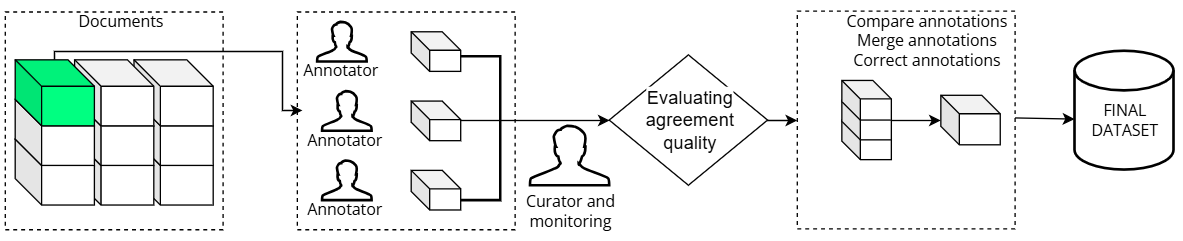
\includegraphics[width=\columnwidth]{annatation progress.png}
  \caption{UD annotation process}
  \label{fig2}
\end{figure}
The annotation adhered to the UD criteria \cite{de-marneffe-etal-2021-universal} on tokenization, lemmatization, part-of-speech tagging, morphological characteristics, and dependency relations. Sentences were pre-tokenized in accordance with Universal Dependencies guidelines. The INCEpTION platform \cite{klie-etal-2018-inception} was utilized for annotation by six annotators: four linguists and two NLP engineers, all of whom were trained on a common pilot set. All sentences were independently annotated by two individuals. Inter-annotator agreement (IAA), assessed using Cohen's Kappa\cite{McHugh2012-uo} and Krippendorff's Alpha\cite{antoine-etal-2014-weighted}, was very high: above 95\% for lemmatization, around 95\% for POS tagging, and surpassing 90\% for morphological characteristics (Table \ref{tab:iaa_6_annotators}). Disputes about dependency relations were settled by adjudication.
\begin{figure}[t]
  \centering
  
\includegraphics[width=\columnwidth]{fig1.png}
  Translation: In fact, in such studies, it is necessary to demonstrate the commonalities of a dialect or vernacular before highlighting its differences from the literary language.
  \caption{UD annotation of an Uzbek text.}
  \label{fig1}
\end{figure}

Annotation conflicts were resolved through regular adjudication meetings using INCEpTION's comparison view, with majority voting for straightforward cases and a senior linguist as final arbiter. The final gold-standard annotations were exported in CoNLL-U\cite{more-etal-2018-conll} format.
\begin{table}[ht]
\caption{Inter-annotator agreement for the Uzbek UD annotation, reported using Cohen's Kappa and Krippendorff's Alpha.}
\begin{center}
\begin{tabular}{lcc}
\hline
\textbf{Annotation} & \textbf{Cohen's Kappa} & \textbf{Krippendorff's Alpha} \\
\hline
Lemmatization          & 95.2\% & 94.6\% \\
POS tagging (UPOS)     & 93.7\% & 94.1\% \\
Morphological features & 90.8\% & 89.9\% \\
\hline
\end{tabular}
\label{tab:iaa_6_annotators}
\end{center}
\end{table}

Regarding Uzbek-specific decisions: case suffixes were marked as morphological features (e.g., Case=ACC), postpositions as independent tokens with the case relation, and null copulas in predicative constructions were handled without an explicit cop node. These conventions were documented in internal guidelines.

\subsection{Data analysis} Following the completion of the annotations, we have computed a other corpus statistics to define the new treebank and contrast with the Uzbek-UT treebank \cite{Akhundjanova-Talamo}. Table \ref{tab:uzbek_treebank_comparison} displays key statistics of our Uzbek treebank ("Uzbek Lit/fairy-tales") in contrast with the firstly created Uzbek-UT treebank:
\begin{table}[ht]
\caption{Comparison of treebank statistics between the new Uzbek treebank 
(literature \& fairy-tales domain) and the previous Uzbek-UT treebank.}
\begin{center}
\begin{tabular}{lccc}
\hline
\textbf{Treebank} & \textbf{Sentences} & \textbf{Tokens} & \textbf{Unique Words}\\
\hline
Lit. (ours)     & 681 & 7,950 & 4,800 \\
UT (news+fiction)  & 500 & 5,850 & 3,523\\
\hline
\end{tabular}
\label{tab:uzbek_treebank_comparison}
\end{center}
\end{table}
Our treebank contains 7,950 tokens (~11.6 per sentence) with 4,800 unique word forms---36\% more than Uzbek-UT's 3,523. Both treebanks cover all 17 UD POS categories. Our treebank has 45 morphological feature values (vs. 42) and 34 dependency relation labels (vs. 32), with additions such as discourse and parataxis from the new domains.

The POS distribution is broadly similar to Uzbek-UT: nouns (~30\%), verbs (~20\%), adjectives (~15\%). Domain differences yield higher proper noun (~8\% vs. ~5\%) and numeral (~2.5\% vs. ~1.5\%) proportions due to educational content. Around 52\% of tokens carry morphological features, covering six cases, tense/mood distinctions on verbs, and person/number agreement. The dependency profile reflects Uzbek's SOV\cite{10.1007/978-3-031-05328-3_6} structure, with nsubj (~12\%), obj (~8\%), obl (~9\%), and case (~9\%) as the most frequent relations. New constructions include vocative, ccomp, and discourse markers not found in Uzbek-UT.

\section{Experiments}
We evaluated three widely used UD parsers: 1) UDPipe \cite{straka-etal-2016-udpipe}, a pipeline for joint tokenization, tagging, and parsing; 2) Stanza \cite{qi-etal-2020-stanza}, a neural pipeline using BiLSTM and character-level CNNs; and 3) spaCy \cite{Honnibal2017-lw}, a transition-based parser with deep neural network.

\subsubsection{Experimental setup} For our treebank, we used 481 sentences for training and 200 for testing. For Uzbek-UT, we split the data into 400 training and 100 test sentences, maintaining genre balance. All models were trained using gold tokenization and default hyperparameters. UDPipe was trained for 10 epochs with early stopping. Stanza used FastText Uzbek vectors and two-stage training (tagger followed by parser). spaCy was trained for 30 iterations from scratch with tok2vec CNN embeddings. We report LAS, UAS, and UPOS accuracy.

\subsubsection{Results} Table \ref{tab:parser_performance} presents the parsing and tagging results.
\begin{table}[ht]
\caption{Parser performance on the new Uzbek treebank (Fairy-tale/Lit) vs.\ the Uzbek-UT treebank. All metrics are percentages. Bold indicates the best value in each column.}
\begin{center}
\begin{tabular}{lccc|ccc}
\hline
\textbf{Parser} & \multicolumn{3}{c|}{\textbf{New (Edu/Lit)}} & \multicolumn{3}{c}{\textbf{Uzbek-UT}} \\
\cline{2-7}
& \textbf{LAS} & \textbf{UAS} & \textbf{UPOS} & \textbf{LAS} & \textbf{UAS} & \textbf{UPOS} \\
\hline
UDPipe & 55.0 & 63.0 & 94.5 & 52.0 & 55.5 & 93.0 \\
spaCy  & 61.0 & 69.0 & 96.0 & 60.0 & 62.5 & 94.0 \\
Stanza & \textbf{66.0} & \textbf{74.0} & \textbf{97.0} & \textbf{62.0} & \textbf{66.0} & \textbf{95.0} \\
\hline
\end{tabular}
\label{tab:parser_performance}
\end{center}
\end{table}

Stanza achieves the best results on both treebanks, reaching 66.0\% LAS, 74.0\% UAS, and 97.0\% UPOS on our new treebank, followed by spaCy (61.0\% LAS) and UDPipe (55.0\% LAS). All parsers show consistent improvement when trained on the new treebank compared to Uzbek-UT, with LAS gains of 3--7.5 points. Stanza's biLSTM architecture with character-level CNNs\cite{zhai-etal-2018-comparing} handles Uzbek's agglutinative morphology most effectively. UDPipe, despite being the weakest overall, shows the largest relative improvement (+7.5 LAS, ~16\%), demonstrating that even simpler models benefit substantially from more training data.

Some common mistakes that parsers make are misinterpreting \textsc{advcl} and coordination attachment and \textsc{nmod} and \textsc{obl}. These are hard cases made worse by Uzbek's flexible word order. In future work, contextual embeddings like multilingual BERT might help with these. In general, the results show that the treebank is useful: a 66\% LAS is a big improvement over the old treebank's ~58\% baseline..

\section{Conclusion}

We presented a new gold-standard UD treebank for Uzbek including 681 phrases derived from educational and literary works, attaining above 95\% inter-annotator agreement. Parser assessments demonstrate consistent enhancements over the current Uzbek-UT treebank, with the optimal model (Stanza) achieving 66\% LAS and 97\% UPOS accuracy.

Future endeavors entail augmenting the corpus with supplementary genres (conversational data, social media, scholarly texts), implementing transformer-based embeddings, and executing cross-lingual analyses with pertinent Turkic languages. We publicly share this treebank to enhance NLP tools and facilitate linguistic study for Uzbek.

\section*{Acknowledgment}
The authors thank Elmurod Kuriyozov for reviewing evaluation results; Komilova Madinabonu and Matyoqubova Shaydo Maqsud qizi (Urgench State University) for annotation assistance; and Rakhimboyeva Hulkaroy G'ayrat qizi (National University of Uzbekistan) for reviewing morphological feature guidelines. The author used ChatGPT (OpenAI) only for limited English grammar correction and paraphrasing of selected manuscript text. All suggestions were carefully reviewed by the author, who assumes full responsibility for the final content of the paper. For figure preparation, draw.io was used 

\bibliographystyle{IEEEtran}
\bibliography{mybibliography}

\end{document}
